\documentclass[a4paper, 10pt]{article}

\usepackage[slovene]{babel}
\usepackage[utf8]{inputenc}
\usepackage[T1]{fontenc}
\usepackage{lmodern}
\usepackage{amsmath}
\usepackage{amsfonts}
\usepackage{amssymb}
\usepackage{enumitem}
\usepackage{epsdice}
\usepackage{array}
\usepackage[table]{xcolor}
\usepackage{makecell}
\usepackage{hyperref}

\newcolumntype{P}[1]{>{\centering\arraybackslash}p{#1}}

\begin{document}

\title{\textbf{\LARGE{Kratko poročilo}}}
\author{Karolina Šavli}
\date{5.\ 4.\ 2024}

\maketitle

% =======================================================================================================================

\noindent V projektni nalogi bom pod mentorstvom GEN-I analizirala in napovedovala odjem električne energije 
\textbf{gospodinjskih odjemalcev}. V analizo niso vključeni samooskrbni odjemalci, torej tisti, 
ki ima sončno elektrarno. Gre za obravnavo časovne vrste: odjema električne energije skozi čas. \\

\noindent Glavni cilj projekta je sestaviti metodo, model, ki bo napovedal odjem za celotni naslednji dan (za naslednjih 24 ur), glede na temperaturo in sevanje. \\

\noindent Podjetje GEN-I je pripravilo tabelo podatkov, sestavljeno iz sedem stolpcev:
\begin{itemize}
    \item  \texttt{DateTimeStartUTC}: univerzalni koordinirani čas,
    \item  \texttt{DateTimeStartCET}: srednjeevropski čas,
    \item  \texttt{Odjem ACT}: neto odjem električne energije v kWh,
    \item  \texttt{Temperatura ACT}: dejanska temperatura, 
    \item  \texttt{Temperatura FC}: napovedana temperatura,
    \item  \texttt{Sevanje ACT}: dejansko sevanje in
    \item  \texttt{Sevanje FC}: napovedano sevanje. 
\end{itemize}

\noindent Uporabljala bom vse stolpce, razen stolpca \texttt{DateTimeStartUTC}, saj v 
okviru časa ključen stolpec \texttt{DateTimeStartCET}.  \\

\noindent Gre za dejanske podatke, ki so bili zaradi varnosti malce prilagojeni. \\

\noindent Odjem je podan za odboje od $1$. novembra $2021$ do $12$. februarja $2024$, na vsakih $15$ minut. Vsega skupaj je $80063$ enot podatkov. 


\begin{figure}[h!]
    \centering
    \caption{Podatki (Vir: GEN-I)}\par\medskip
    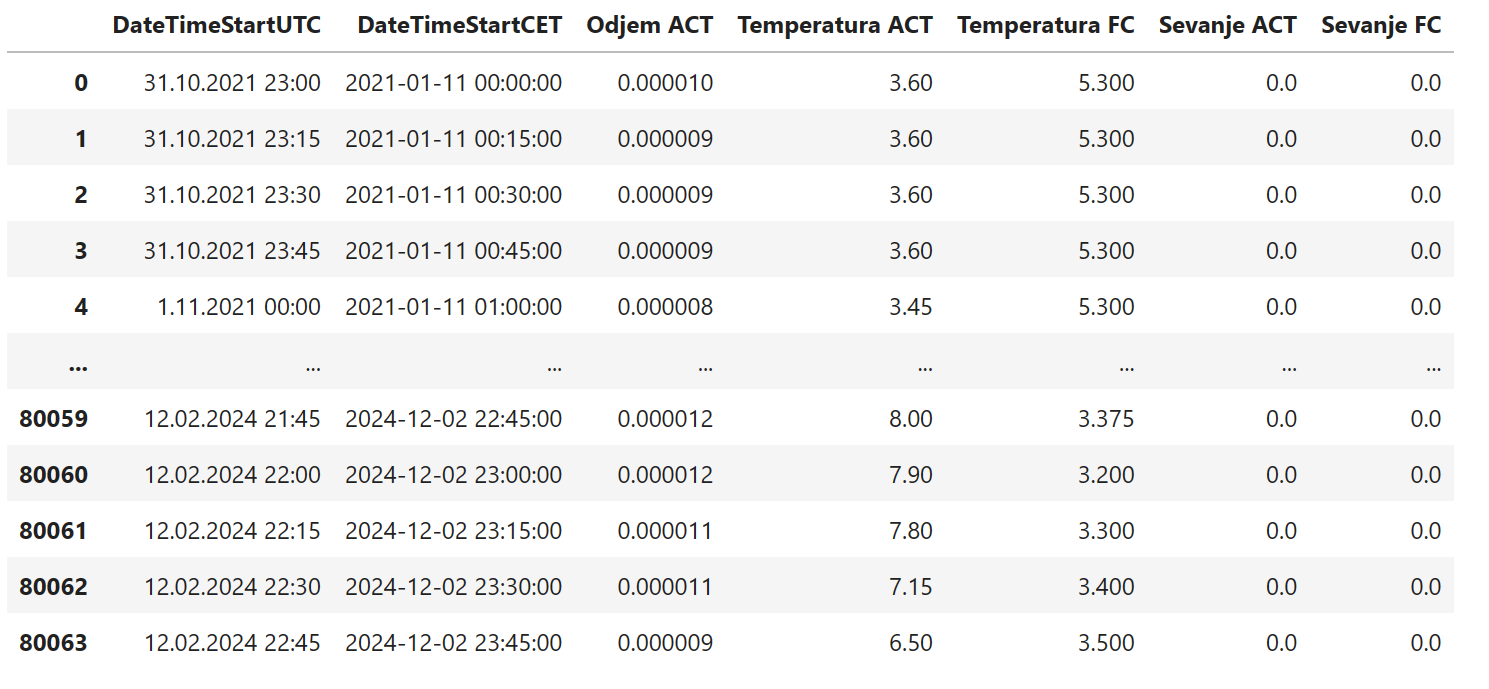
\includegraphics[width=0.95\textwidth]{tabela.png}
\end{figure}



Analiza in napovedovanje bo izvedeno v programskem jeziku Python.

Poglejmo si odjem, in sicer za leti $2022$ in $2023$. Zaradi boljše preglednosti sem za vsak dan povprečila vse podatke odjema.


\begin{figure}[h!]
    \centering
    \caption{Podatki (Odjem električne energije, 2022-2023)}\par\medskip
    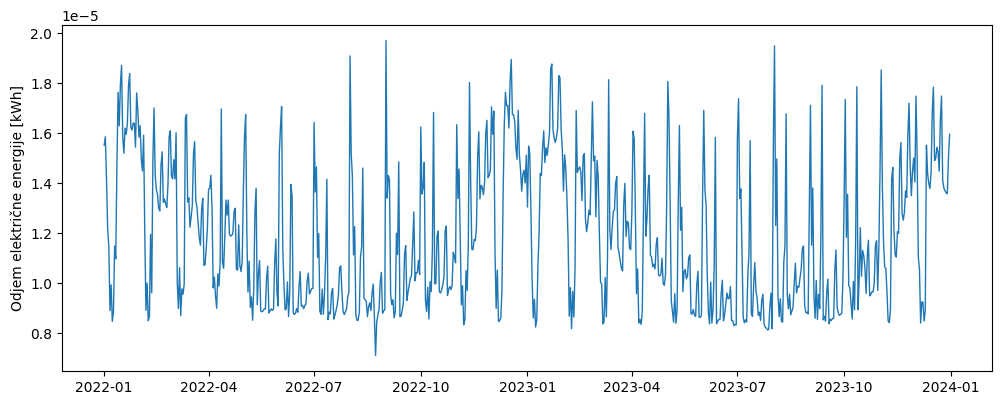
\includegraphics[width=0.95\textwidth]{output.png}
\end{figure}



\noindent Opaziti je sezonskost; večji odjem v zimskih mesecih, kar je pomembno pri 
načrtovanju in upravljanju proizvodnje in distribucije električne energije. 
V zimskih mesecih je odjem višji, zaradi ogrevanja, razsvetljave, saj se število ur 
dnevne svetlobe podaljša in nasploh se poveča uporabe električnih aparatov, k
ot so grelniki, sušilniki in podobno.  \\

\noindent Torej na odjem električne energije očitno vplivajo temperature, 
ki jih imamo za potrebe analize podane v tabeli. Imamo pa tudi podatek 
sevanja, ki pričakujem, da ne bo pomemben v moji analizi, saj le-ta ne 
vključuje odjemalcev, ki imajo sončno elektrarno. Mogoče pa bo vseeno 
imel nekaj vpliva, saj močna sončna svetloba povzroči povečano porabo 
električne energije za hlajenje, ker se ljudje zatekajo k napravam za 
hlajenje prostorov. \\

\noindent Po potrebi bom uporabila še kakšne druge dejavnike. S strani GEN-I 
predlagana stran za pridobitev dodatnih podatkov je \href{https://ot.borzen.si/Domov/Podatki-trga/Koli%C4%8Dine-in-zneski-izravnave}{Borzen}

\end{document}